\documentclass[12pt,a4paper]{report}
\usepackage{textcase}
\usepackage[utf8]{vietnam}
\usepackage[latin1]{inputenc}
\usepackage{fancybox}
\usepackage{amsmath}
%\usepackage{amsthm}
\usepackage{amsfonts}
\usepackage{amssymb}
\usepackage{graphicx}
\usepackage{enumerate}
\usepackage{wrapfig}
\usepackage{color, fancyhdr, graphicx, wrapfig}
\usepackage{subfig}
\usepackage[unicode]{hyperref}
\usepackage[left=3.5cm,right=2cm,top=3.5cm,bottom=2cm]{geometry}
\usepackage[thref,thmmarks,standard,amsmath,hyperref]{ntheorem}
\renewcommand{\baselinestretch}{1.5}

%Môi trường Nhận xét
\theoremstyle{plain} 
\theoremheaderfont{\bfseries} 
\theorembodyfont{\slshape} 
\theoremseparator {.}      
\theoremsymbol{\NoEndMark}
\renewtheorem{remark}{Nhận xét}[chapter] 
\newcommand{\nhx}[1]{\begin{remark}#1\end{remark}}
%Môi trường Hệ quả
\theoremstyle{plain} 
\theoremheaderfont{\bfseries} 
\theorembodyfont{\slshape} 
\theoremseparator {.}         
\theoremsymbol{\NoEndMark} 
\renewtheorem{Corollary}{Hệ quả}[chapter] 
\newcommand{\hq}[1]{\begin{Corollary}#1\end{Corollary}}
%Môi trường Định nghĩa
\theoremstyle{plain} 
\theoremheaderfont{\bfseries} 
\theorembodyfont{\slshape} 
\theoremseparator {.}      
\theoremsymbol{\NoEndMark} 
\renewtheorem{definition}{Định nghĩa}[chapter] 
\newcommand{\dng}[1]{\begin{definition}#1\end{definition}}
%Môi trường Định nghĩa
\theoremstyle{plain} 
\theoremheaderfont{\bfseries} 
\theorembodyfont{\slshape} 
\theoremseparator {.}      
\theoremsymbol{\NoEndMark} 
\renewtheorem{theorem}{Định lý}[chapter] 
\newcommand{\dly}[1]{\begin{theorem}#1\end{theorem}}
%Môi trường Chứng minh
\theoremstyle{plain} 
\theoremheaderfont{\bfseries\slshape} 
\theorembodyfont{\normalfont} 
\theoremseparator{.}
\theoremsymbol{\ensuremath{_\square}}
\renewtheorem{proof}{Chứng minh định lý}[chapter] 
\newcommand{\chm}[1]{\begin{proof}#1\end{proof}}
%Môi trường Tính chất
\theoremstyle{plain} 
\theoremheaderfont{\bfseries} 
\theorembodyfont{\slshape} 
\theoremseparator {.}      
\theoremsymbol{\NoEndMark} 
\renewtheorem{properties}{Tính chất}[chapter] 
\newcommand{\tch}[1]{\begin{properties}#1\end{properties}}
%--------------new enviroment only------------------
\newenvironment{my-itemize}
	{\begin{minipage}[t]{0.95\linewidth}\begin{itemize}}
	{\end{itemize}\end{minipage}}
\newenvironment{my-enumerate}
	{\begin{minipage}[t]{0.8\linewidth}\begin{enumerate}}
	{\end{enumerate}\end{minipage}}
\usepackage{tikz}
\usepackage{wrapfig}



% Ghi tắt một số ký hiệu
\newcommand{\ssubsection}[1]{\subsubsection{\hspace{4pt}\large\normal{#1}}}
\newcommand{\itembf}[1]{\item\textbf{#1}}

\newcommand{\Real}{\mathbb{R}}
\newcommand{\Laplace}{\mathcal{L}}

\usepackage[unicode]{hyperref}
\usepackage{indentfirst}
\usepackage[inline]{enumitem}
%\usepackage{paralist}
\author{Nguyen Thien Dong}
\pagestyle{fancy}
    \lhead{\it }
    \rchapter
    \lfoot{\it Nhóm 22}
    \rfoot{\it Các mô hình ngẫu nhiên}
    \renewcommand{\headrulewidth}{1,2pt}
    \renewcommand{\footrulewidth}{1,2pt}
\pagenumbering{arabic}
\setcounter{page}{1}
\include{chapter} 
\begin{document}
\fontsize{14pt}{18pt}\selectfont % Lệnh thay đổi cỡ chữ thành cỡ 13, cỡ dòng 18 (theo quy chuẩn của Khóa Luận TN).

\setlength{\baselineskip}{18truept}
\newpage
\begin{document}
\fontsize{14pt}{18pt}\selectfont % Lệnh thay đổi cỡ chữ thành cỡ 13, cỡ dòng 18 (theo quy chuẩn của Khóa Luận TN).
\pagenumbering{gobble}
 
\chapter*{Lời nói đầu}
\addcontentsline{toc}{chapter}{{\bf Lời nói đầu}\rm}
\thispagestyle{empty}
\newline \par 
Trong thực tế, nhiều khách hàng phải xếp thành hàng để đợi mua vé, các cuộc gọi điện thoại phải đợi để được liên lạc tại các tổng đài điện thoại và các tác vụ có thể phải đợi để nhận được điều khiển của CPU trong các máy tính. Trong một mạng máy tính, nhiều người cùng chia sẻ tài nguyên nhưng chỉ có thể sử dụng tài nguyen cho mỗi công việc tại mỗi thời điểm, vì thế các công việc khác phải xếp xếp hàng. Các gói tin có thể phải đợi trong các bộ đệm tại một nút mạng nào đó trên mạng máy tính. Tất cả các ví dụ trên đã và đang được nghiên cứu nhờ sử dụng một lý thuyết toán học của các xếp hàng có tên là lý thuyết xếp hàng (lý thuyết hàng chờ). Lý thuyết xếp hàng giúp ta xác định được các số đo hiệu năng của các hàng xếp.
\par Lý thuyết xếp hàng có nguồn gốc từ đầu thế kỷ 20 với các nghiên cứu khởi đầu của nhà toán học người Đan Mạch A. K. Erlang trên các mạng điện thoại và sự sáng tạo của các mô hình Markov do nhà toán học người Nga A. A. Markov. Ngày nay lý thuyết xếp hàng được sử dụng rộng rãi cho các ứng dụng khác nhau và nó vẫn đang được nghiên cứu và phát triển.
\par Lý thuyết này có thể áp dụng vào giải quyết các bài toán kinh tế, những bài toán phụ thuộc vào các yếu tố ngẫu nhiên. Lý thuyết này cũng phù hợp với các kiến thức cơ sở của môn học "Các mô hình ngẫu nhiên và ứng dụng" do cô giáo TS Nguyễn Thị Ngọc Anh trực tiếp giảng dạy.
Vì vậy, em đã chọn đề tài "Áp dụng lý thuyết xếp hàng vào giải quyết bài toán Bán vé tàu" để làm đề tài nghiên cứu cho bản thân. Nội dung chính của tiểu luận gồm:
\par \textit{Chương 1: Giới thiệu lý thuyết hàng chờ}
\par \textit{Chương 2: Giải quyết bài toán bán vé tàu}
\par \textit{Chương 3: Chương trình}
\par Do khả năng có hạn nên tiểu luận không tránh khỏi những thiếu sót và hạn chế. Rất mong nhận được sự góp ý và chỉ bảo của Cô giáo để nhóm có thể hoàn chỉnh hơn nữa những hiểu biết của mình.
\end{my-itemize}

\pagestyle{empty}
}
\tableofcontents{
\cleardoublepage
	\pagestyle{empty}}

\setcounter{page}{1}
\pagenumbering{arabic}
\chapter{Kiến thức cơ sở}
\section{Biến ngẫu nhiên}
Biến ngẫu nhiên là một khái niệm quan trọng trong xác suất thống kê. Một cách
giản lược, biến ngẫu nhiên còn gọi là đại lượng ngẫu nhiên, được hiểu là biến nhận
giá trị tùy thuộc vào kết quả của phép thử (phép đo, quan sát, thí nghiệm) mà không
thể đoán trước được.
 \par Biến ngẫu nhiên chia làm hai loại: rời rạc và liên tục. Biến rời rạc là biến ngẫu
nhiên nhận các giá trị từ một tập hợp hữu hạn hoặc đếm được. Biến liên tục là biến
ngẫu nhiên nhận giá trị trên một tập con liên tục của tập số thực.
\section{Phân phối Poisson}
\subsection{Định nghĩa}
\dng{
Một biến ngẫu nhiên X được gọi là có phân bố Poisson với tham số $\lambda > 0$, ký hiệu: $X \sim \rho(X)$, nếu $X$ có hàm trọng số xác suất:
\[P_X(x)=P(X = x) = \frac{\lambda_x}{x!} e^{-\lambda}\;\;, \quad x = 0,1,...\]
}
\subsection{Giá trị đặc trưng của phân phối Poisson}
\begin{itemize}
    \item Kỳ vọng:
\begin{align*}
    E(X)&=\displaystyle\sum_{x=0}^{+\infty}x.P_X(x)=\displaystyle\sum_{x=0}^{+\infty}x.\frac{\lambda^x}{x!} e^{-\lambda}\\
    &= \displaystyle\sum_{x=0}^{+\infty}\frac{\lambda^x}{(x-1)!} e^{-\lambda} = \lambda.e^{-\lambda} \displaystyle\sum_{x=0}^{+\infty}\frac{\lambda^{x-1}}{(x-1)!}
\end{align*}
Đặt $n=x-1$, ta có:
\[E(X) = \lambda.e^{-\lambda} \displaystyle\sum_{x=0}^{+\infty}\frac{\lambda^n}{n!}= \lambda.e^{-\lambda}.e^\lambda = \lambda\]
\item Phương sai:
\begin{align*}
    V(X) &= E(X^2) -(E(X))^2 = E(X^2) - \lambda^2\\
    E(X^2) &= \displaystyle\sum_{x=0}^{+\infty}x^2.\frac{\lambda^x}{x!} e^{-\lambda} = \lambda^2 + \lambda\\
    V(X) &= \lambda^2 + \lambda - \lambda^2 = \lambda
\end{align*}
\end{itemize}
\section{Phân phối mũ}
\subsection{Định nghĩa}
\dng{
Biến ngẫu nhiên $X$ được gọi là có phân phối mũ với tham số $\mu > 0$, ký hiệu: $X \sim Exp(\mu)$ và hàm mật độ có dạng:
\begin{align*}f_X(x)=
    \begin{cases}
    \mu.e^{-\mu x}\;&, \quad x \ge 0\\
    0&, \quad x<0
    \end{cases}
\end{align*}
}
\subsection{Hàm phân phối xác suất}
Hàm phân phối xác suất được định nghĩa bởi hàm sau:
\[F_X(x) = P(X<x) = \displaystyle\int_{-\infty}^{+\infty}f_X(t)dt\]
\begin{itemize}
    \item $x<0: F_X(x)= \displaystyle\int_{-\infty}^{+\infty}0dt = 0$
    \item $x \ge 0: F_X(x)= \displaystyle\int_{-\infty}^00dt + \displaystyle\int_{0}^x \mu.e^{-\mu x}dt = 0 - e^{-\mu t}|_0^x = - e^{-\mu x} + 1$
\end{itemize}
Vậy $F_X(x)=
\begin{cases}
    1 - e^{-\mu x}\;&, \;\;x \ge 0\\
    0 &, \;\;x < 0
\end{cases}$
\subsection{Các giá trị đặc trưng}
\begin{itemize}
    \item Kỳ vọng:
    \[E(X) = \displaystyle\int_{-\infty}^{+\infty}x.f_X(x)dx = \displaystyle\int_{-\infty}^0 x.0dx + \displaystyle\int_{0}^{+\infty} x.e^{-\mu x}dx = \frac{1}{\mu}\]
    \item Phương sai:
    \[V(X) = E(X^2) -(E(X))^2 = \displaystyle\int_{0}^{+\infty} x^2.e^{-\mu x}dx - \frac{1}{\mu^2} = \frac{2}{\mu^2}-\frac{1}{\mu^2}=\frac{1}{\mu^2}\]
\end{itemize}
\chapter{Lý thuyết xếp hàng}
\section{Giới thiệu chung}
Lý thuyết xếp hàng là một trong các công cụ toán học mạnh mẽ cho việc phân tích, ước lượng trong các hệ thống xếp hàng. Lý thuyết xếp hàng thông thường được áp dụng cho các hệ thống lý tưởng để đưa ra các kết quả gần đúng cho một mô hình thực tế. Tính chất chung của các giải pháp ứng dụng lý thuyết xếp hàng là làm rõ lưu lượng dòng vào, để cung cấp dự báo nhứng danh giới lớn hơn trên những kết quả nghiên cứu thu được. Chúng rất hữu ích cho việc xác định tính đúng đắn của các phương pháp.

\section{Định nghĩa}
Lý thuyết xếp hàng là một phần của lý thuyết xác suất thống kê, nó được định nghĩa là một bộ các quy tắc và luật đề cập đến việc tắc nghẽn và phương pháp giải quyêt tắc nghẽn như: dự đoán độ trễ, trễ nhỏ nhất, độ dài hàng chờ, số kênh phục vụ cần thiết,... Lý thuyết xếp hàng có rất nhiều ứng dụng từ việc nghiên cứu xe cộ lưu thông trên đường phố, phục vụ khách hàng tại các siêu thị, nhà hàng...
\par Một quá trình xếp hàng là:
\par\begin{my-itemize}
    \item Dòng khách hàng tới
    \item Khả năng phục vụ của server
    \item Nếu khách hàng tới chưa được phục vụ thì sẽ xếp hàng chờ
    \item Hệ thống xếp hàng gồm khách hàng trong xếp hàng và khách hàng đang được phục vụ.
\end{my-itemize}\\
\par Chuẩn ký hiệu cho hệ thống xếp hàng được sắp xếp như sau\\
Dòng vào / dòng phục vụ / số lượng server / số lượng khách hàng lớn nhất trong hệ thống / quy tắc xếp hàng.
\par\begin{my-itemize}
    \item Dòng vào: lượng khách tới hệ thống, \item Dòng phục vụ: lượng khách được phục vụ xong ra khỏi server, 
    \item Số server: số kênh phục vụ, 
    \item Lượng khách lớn nhất: tổng lượng khách đang phục vụ và trong hàng chờ, \item Quy tắc xếp hàng: Một số nguyên tắc phục vụ thường được áp dụng trong các hệ thống xếp hàng là FIFO (First in first out), LIFO (Last in first out), FCFS (First come first serve), có ưu tiên, không ưu tiên, Random Order...
\end{my-itemize}\\
\par Trong các hệ thống hàng chờ thường xuyên diễn ra hai quá trình: quá trình này sinh các yêu cầu (một yêu cầu còn được coi là một tín hiệu cần được phục vụ) và quá trình phục vụ các yêu cầy ấy. Song trong quá trình phục vụ của các hệ thống, do nhiều nguyên nhân khác nhau, thường xảy ra các tình trạng sau: Trong nhiều trường hợp, quá trình phục vụ không đáp ứng các yêu cầu và do đó dẫn đến kết quả là nhiều yêu cầu phải chờ để được phục vụ. Ngược lại, trong một số tình huống khác, khả năng phục vụ của hệ thống vượt quá số yêu cầu cần được phục vụ, với kết quả là hệ thống không sử dụng hết phương tiện phục vụ.
\par Người quản trị hệ thống phải xác định cho được những chi phú vô ích. Những chi phí vô ích này tạo thành tính không hiệu quả của hệ thống. Có hai dạng chi phí vô ích:\\
\begin{my-itemize}
\item Chi phí của khách hàng phải chờ trong hệ thống trước khi được phục vụ. Chi phí này có thể hiểu được một cách tương đương là trong cùng một khoảng thời gian quản lý T, nếu khách hàng chờ lâu thì lượng khách hàng chờ tới trong khoảng thời gian T giảm.
\item Chi phí cho các trạm phục vụ khách hàng nhưng lại không có khách hàng. Như vậy trong khoảng thời gian quản lý T, tỷ lệ thời gian phục vụ khách hàng tạo thành hiệu suất U của một trạm phục vụ. Hiệu suất càng gần 1 thì chi phí vô ích càng nhỏ và ngược lại, nếu hiệu suất gần bằng 0 thì chi phí vô ích càng lớn.
\end{my-itemize}\\
\par Đây là hai loại chi phí ngược nhau: nếu giảm chi phí vô ích từ phía khách hàng tức là giảm thời gian chờ của khách hàng thì phải tăng số trạm phục vụ; và như vậy làm tăng chi phí vô ích từ phía phục vụ. Ngược lại nếu muốn giảm chi phí vô ích từ phía phục vụ thì phải giảm số trạm phục vụ nhưng điều này lại làm tăng thời gian chờ của khách hàng. Rõ ràng muốn tăng tính hiệu quả hoạt động của hệ thống thì cần phải cân đối tổng thể từ hai loại chi phí này.
\par Vì vậy bài toán đặt ra là:\par
\begin{my-itemize}
\item Phân tích bản chất của quá trình diễn ra trong các hệ thống hàng chờ và thiết lập các mối liên hệ về lượng giữa các đặc trưng của các quá trình ấy. Điều đó có nghĩa là cần thiết lập hay lựa chọn một mô hình hàng chờ phản ánh được bản chất của hệ thống.
\item Trên cơ sở các mối liên hệ đã được xây dựng và các số liệu thu được từ hệ thống, cần tính toán, phân tích và đưa ra các quyết định nhằm tìm ra các giá trị thích hợp cho các tham số điều khiển / thiết kế của hệ thống để thiết kế hay điều khiển các hoạt động của hệ thống hoạt động một cách có hiệu quả hơn.
\end{my-itemize}
\section{Các phương pháp giải mô hình hàng chờ}
Để tìm lời giải cho một mô hình hàng chờ người ta thường sử dụng hai phương pháp: phương pháp giải tích và phương pháp mô phỏng trên máy tính. 
\par Phương pháp giải tích để giải mô hình hàng chờ gồm các bước sau:\par
\begin{my-itemize}
\item Bước 1: Phân tích hệ thống, chủ yếu là phân tích bản chất của dòng yêu cầu / tín hiệu đến và các trạng thái của hệ thống. 
\item Bước 2: Thiết lập hệ phương trình trạng thái cho các xác suất trạng thái (xác suất để hệ thống ở một trạng thái nào đó tại thời điểm t). 
\item Bước 3: Giải hệ phương trình để tìm các xác suất trạng thái. Từ đó thiết lập các mối quan hệ giữa các chỉ tiêu cần phân tích.
\item Bước 4: Tính toán, phân tích các chỉ tiêu, trên cơ sở đó đưa ra các nhận xét và các quyết định.
\end{my-itemize}\\
\par Phương pháp giải tích thường sử dụng các giả thiết rất chặt chẽ của Toán học về các đặc trưng của hệ thống, vì vậy nó có một số hạn chế nhất định khi giải các bài toán thực tế.
\par Trong khi đó, phương pháp mô phỏng / mô phỏng ngẫu nhiên để giải mô hình hàng chờ được áp dụng cho các bài toán dịch vụ đám đông không giải được bằng công cụ giải tích, nhất là liên quan đến hệ thống lớn, bất ổn định, hàm chứa nhiều yếu tố ngẫu nhiên, không tuân theo các giả thiết quá chặt chẽ của Toán học. Trong nhiều trường hợp phương pháp mô phỏng cho ta tiết kiệm được thời gian và chi phí nghiên cứu. Tuy phương pháp mô phỏng chỉ tạo ra các phương án đủ tốt để đánh giá hoạt động của hệ thống chứ không đưa ra được kĩ thuật tìm lời giải tốt nhất, nó tỏ ra rất thành công khi giải quyết nhiều bài toán hàng chờ nảy sinh từ thực tiễn. 
\par Các bước cần tiến hành khi áp dụng phương pháp mô phỏng bao gồm:\par
\begin{my-itemize}
\item Bước 1: Xác định bài toán hay hệ thống hàng chờ cần mô phỏng và mô hình mô phỏng. 
\item Bước 2: Đo và thu thập số liệu càn thiết để khảo sát thống kê các số đặc trưng / các yếu tố cơ bản của mô hình. 
\item Bước 3: Chạy mô phỏng kiểm chứng (test simulation) mô hình và so sánh kết quả kiểm chứng với các kết quả đã biết được trong thực tế. Phân tích kết quả chạy mô phỏng kiểm chứng, nếu cần thì phải sửa lại phương án đã được đánh giá qua chạy mô phỏng.
\item Bước 4: Chạy mô phỏng để kiểm chứng phương án cuối cùng và kiểm tra tính đúng đắn của mọi kết luận về hệ thống thực tế được rút ra sau khi chạy mô phỏng. Triển khai hoạt động của hệ thống hàng chờ dựa trên phương án tìm được. 
\end{my-itemize}
\par Từ những phân tích trên đây có thể thấy Lí thuyết hàng chờ (Waiting Line Theory) còn gọi là Lý thuyết hệ phục vụ công cộng hay Lý thuyết hệ dịch vụ đám đông là lĩnh vực rất quan trọng của Toán ứng dụng / Vận trù học. Nhiều bài toán thực tế trong các lĩnh vực hệ thống dịch vụ, kĩ thuật, ...đã được giải quyết thành công nhờ áp dụng phương pháp mô phỏng mô hình hàng chờ.
\section{Các yếu tố cơ bản của hệ thống hàng chờ}
Hệ thống hàng chờ tổng quát được minh họa như hình sau.
\begin{center}
    \begin{figure}[htp]
    \begin{center}
     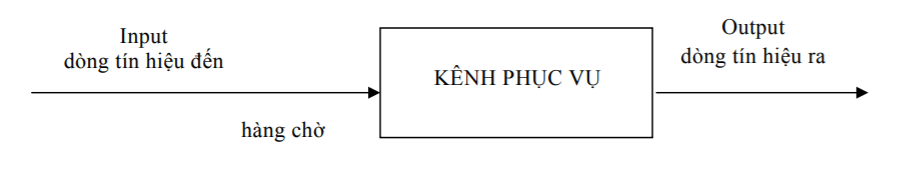
\includegraphics[scale=1]{img/HeThongHangCho.PNG}
    \end{center}
    \caption{Hệ thống hàng chờ}
    \end{figure}
\end{center}
Các yếu tố cơ bản của hệ thống hàng chờ bao gồm
\subsection{Bố trí vật lý của hệ thống}
Hệ thống hàng chờ có một số dạng bố trí vật lí (phisical layout) như minh họa trên hình 2.1.\newpage
\begin{center}
    \begin{figure}[htp]
    \begin{center}
     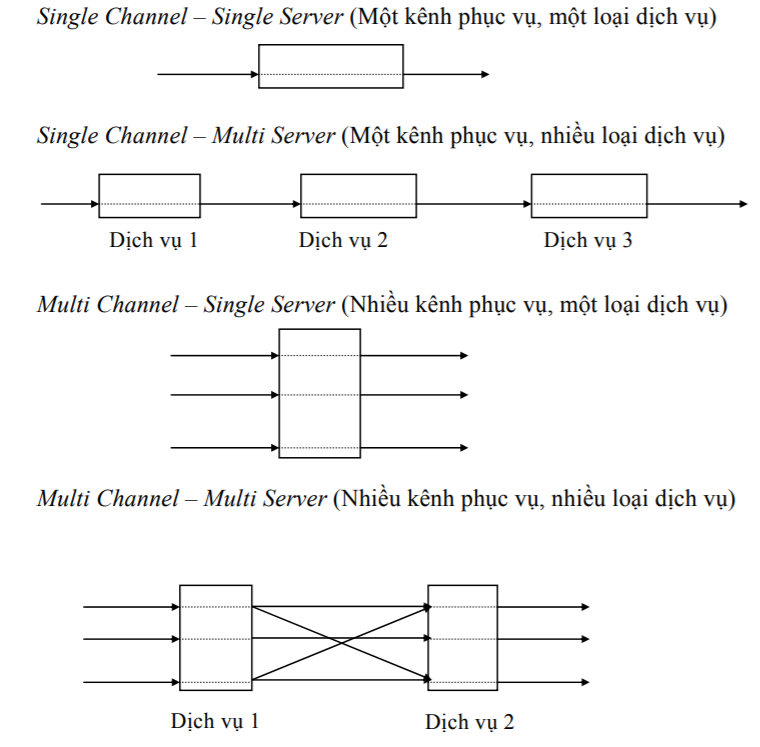
\includegraphics[scale=1]{img/CacDangHTHangCho.PNG}
    \end{center}
    \caption{Các dạng hệ thống hàng chờ}
    \end{figure}
\end{center}
 Trên hình 1.2, các kênh phục vụ được hiểu là những thiết bị kĩ thuật hoặc con người hoặc những tổ hợp các thiết bị kĩ thuật và con người được tổ chức quản lí một cách thích hợp nhằm phục vụ các yêu cầu / các tín hiệu đến hệ thống. Chẳng hạn, ở các trạm điện thoại tự động, kênh phục vỵ là các đường dây liên lạc cùng các thiết bị kĩ thuật khác phục vụ cho việc đàm thoại.
\subsection{Nguyên tắc phục vụ}
Nguyên tắc phục vụ( hay nội quy) của hệ thống là cách thức nhận các yêu cầu vào các kênh phục vụ. Nguyên tắc phục vụ cho biết trường hợp nào thì yêu cầu được nhận vào phục vụ và cách thức phân bố các yêu cầu vào các kênh như thế nào. Đồng thời nguyên tắc phục vụ cũng cho biết trong trường hợp nào yêu cầu bị từ chối hoặc phải chờ và giới hạn của thời gian chờ.
\par Một số nguyên tắc phục vụ thường được áp dụng trong các hệ thống hàng chờ là \par
\begin{my-itemize} 
\item FIFO(First in first out), 
\item LIFO (Last in first out), 
\item FCFS(First come first serve), 
\item Có ưu tiên, 
\item Không ưu tiên,...
\end{my-itemize}
\subsection{Các phân phối xác suất của các dòng tín hiệu, dòng phục vụ}
Số tín hiệu đến trong một khoảng thời gian cũng như thời gian phục vụ từng tín hiệu nói chung là những biến ngẫu nhiên, và do đó, chúng tuân theo các quy luật phân phối xác suất. Các quy luật phân phối xác suất này được thiết lập căn cứ các số liệu thực nghiệm thu thập từ các quan sát, thí nghiệm, hay từ cơ sở dữ liệu sẵn có.
\par Đối với dòng tín hiệu đầu vào, thông thường chúng ta giả sử rằng số tín hiệu đến trong vòng một khoảng thời gian nào đó được ấn định được trước (1 phút, 3 phút, 5 phút, 30 phút,...) tuân theo luật phân phối Poisson $P(\lambda)$. Ở đây, tham số $\lambda$ đặc trưng cho tín hiệu đến (trung bình) là 100 người trong 1 giờ. Có nghĩa là, số khách vào siêu thị là biến ngẫu nhiên $X$ có phân phối Poisson với $\lambda = 100$. Hoặc, với số cuộc gọi (trung bình) đến tổng tài trong vòng 1 phút là 3 (tín hiệu)thì có $X \sim P(3)$. 
\par Một cách chính xác hơn, trong những trường hợp trên, ta có dòng tín hiệu đến là dòng Poisson dừng( còn gọi là dòng tối giản) với các tính chất trên sau:\par
\begin{my-itemize}
    \item \textit{Tính không hiệu quả:} Một dòng tín hiệu có tính không hiệu quả nếu xác suất xuất hiện một số tín hiệu nào đó trong một khoảng thời gian nhất định không phụ thuộc vào việc đã có bao nhiêu tín hiệu đã xuất hiện và xuất hiện như thế nào trước khoảng thời gian đó.
    \item \textit{Tính đơn nhất:} Dòng tín hiệu có tính đơn nhất nếu xét trong khoảng thời gian khá bé thì sự kiện "có nhiều hơn một tín hiệu xuất hiện" hầu như không xảy ra, Về mặt thời gian ta có thể xem dòng tín hiệu có tính đơn nhất nếu thời điểm xuất hiện các tín hiệu không trùng nhau.
    \item \textit{Tính dừng:} Dòng tín hiệu có tính dừng nếu xác suất xuất hiện một số tín hiệu nào đó trong khoảng thời gian $\tau$ chỉ phụ thuộc vào độ dài của $\tau$ chứ không phụ thuộc vào điểm khởi đầu của $\tau$.
\end{my-itemize}
\section{Một số đặc trưng của hệ thống xếp hàng}
Bất kỳ một hệ thống xếp hàng nào cũng được mô tả bởi đăc trưng sau: Quá trình đến: Nếu các khách hàng đến xếp hàng vào các thười điểm $t_1,t_2,...,t_j$ thì các biến số ngẫu nhiên $P_j = t_j −t_{j−1}$ được gọi là các thời điểm giữa các lần đến. Các thời điểm này thường được giả thuyết là các biến số ngẫu nhiên độc lập và được phân bố đồng nhất IID (Independent and Identically Destributed). Các quá trình đến thông dụng nhất là:\par
\begin{my-itemize}
    \item $M =$ quá trình mũ (là quá trình Markov hay quá trình không có bộ nhớ).
    \item $Er (Erlang r) =$ là quá trình Erlang bậc r: trung tâm dịch vụ ở đây được biểu diễn bởi một dãy có r giai đoạn trễ, mỗi giai đoạn có cùng thời gian dịch vụ trung bình và có phân phối mũ. Không có các xếp hàng tại bất cứ môt giai đoạn phục vụ nào vì yêu cầu tiếp theo sẽ không được phuc vụ nếu như yêu cầu trước đó chưa hoàn thành dịch vụ ở tất cả r giai đoạn.
    \item $Hr =$ quá trình siêu số mũ bậc r.
    \item $D =$ quá trình tất định.
    \item $G =$ quá trình chung.
\end{my-itemize}
\section{Một số điểm hạn chế của các mô hình hàng chờ}
Các mô hình hàng chờ giới thiệu ở trên là những mô hình tiện lợi nhất được áp dụng khá rộng rãi. Tuy nhiên, do các mô hình này công nhận các giả thuyết "quá chặt chẽ" ít xảy ra trên thực tế, nên các chuyên gia trong lĩnh vưc Toán ứng dụng/Vận trù học/Khoa học quản lí cũng đã đề xuất xem xét nhiều mô hình khác. Đó là các mô hình với các giả thiết như: số tín hiệu cần phục vụ là hữu hạn, dòng tín hiệu đến là Poisson, cường độ phục vụ phụ thuộc vào số tín hiệu trong hàng chờ ... và việc giải quyết mô hình như vậy cần tới sự trợ giúp của phương pháp mô phỏng ngẫu nhiên.
\par Ngay cả khi các giả thiết khá chặt chẽ của bốn mô hình đã nêu trong mục này (cũng như môt số mô hình tương tự khác) là hợp lí, thì việc các mô hình hàng chờ đưa ra các lời giải với trạng thái vững \textit{(steady state solutions)} cũng ít có ý nghĩa thưc tế. Trong nhiều ứng dụng thưc tiễn. Trong nhiều ứng dụng thực tiễn, các hệ thống hàng chờ không bao giờ đạt tới các trạng thái vững. Chẳng hạn, trong một hệ thống hàng chờ, cường độ tín hiệu dến trung bình thay đổi nhiều lần trong ngày không cho phép hệ thống đạt được trạng thái vững.
\par Do đó, để giải quyết nhiều bài toán hàng chờ trong lĩnh vực dịch vụ đám đông và các lĩnh vực khác, cần áp dụng phương pháp mô phỏng để tìm ra lời giải có tính thực tiễn cho các mô hình hàng chờ khi hệ thống không thể đạt tới trạng thái vững hoặc khi không có các mô hình lí thuyết thích hợp.
\chapter{Áp dụng giải quyết bài toán bán vé tàu}
\section{Phát biểu bài toán}
Giả sử dòng khách hàng đến mua vé tại một ga tàu với M quầy phục vụ là dòng Poisson với tham số $\lambda$ là số khách hàng /1 phút, ví dụ $\lambda = 6$ (có nghĩa là khách hàng đến phòng bán vé với các thời điểm tuân theo luật phân phối mũ tham số $\lambda = 6$). Ngoài ra, còn biết nguyên tắc phục vụ là FCFS (First come first serve) và thời gian phục vụ tại mỗi quầy có luật phân phối mũ với kì vọng $t$ (phút). Suy ra, $\mu = \frac{1}{t}$.

\section{Hệ thống xếp hàng M/M/C/K}
\begin{itemize}
    \item  Có tiến trình đến là một tiến trình phân phối Poisson.
    \item Hệ thống phục vụ có thời gian dịch vụ là một biến ngẫu nhiên phân phối mũ.
    \item $C$ là số trạm phục vụ (server) khách hàng.
    \item $K$ là số lượng khách có thể chứa tối đa trong hệ thống .
\end{itemize}
Hệ thống này được xây dựng bằng cách cho tốc độ đến hoặc tốc độ dịch vụ phụ thuộc vào số các khách hàng trong hệ thống. Ta có sơ đồ biểu diễn hệ thống xếp hàng M/M/C/K như sau:
\begin{center}
    \begin{figure}[htp]
    \begin{center}
     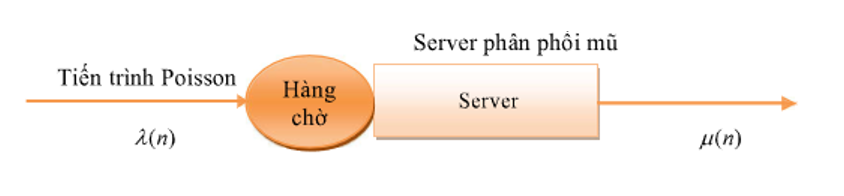
\includegraphics[scale=1]{img/HT_MMCK.PNG}
    \end{center}
    \caption{Sơ đồ biểu diễn hệ thống xếp hàng M/M/C/K.}
    \end{figure}
\end{center}
\par Với mô hình của hệ thống trên ta có lược đồ chuyển trạng thái của mô hình này nhưu sau:
\begin{center}
    \begin{figure}[htp]
    \begin{center}
     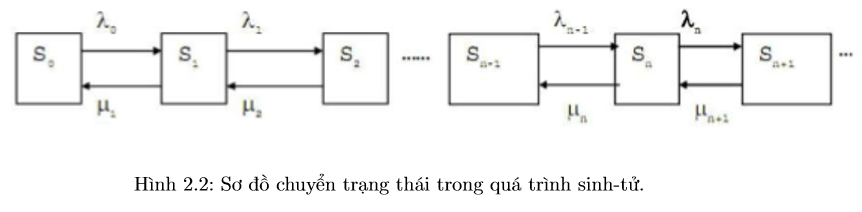
\includegraphics[scale=1]{img/QT_SinhTu.PNG}
    \end{center}
    \caption{Sơ đồ chuyển trạng thái trong quá trình sinh-tử.}
    \end{figure}
\end{center}
\section{Giải quyết bài toán}
Bài toán có $k+1$ trạng thái\[\lambda_i = \lambda, \forall i = 1,2,...,n\]
\begin{align*}
    \mu_n = \begin{cases}
    n\mu, \qquad n=1,2,...,c-1\\
    c\mu, \qquad n=c,c+1,...
    \end{cases}
\end{align*}
Mô hình hệ thống xếp hàng M/M/C/K.
begin{center}
    \begin{figure}[htp]
    \begin{center}
     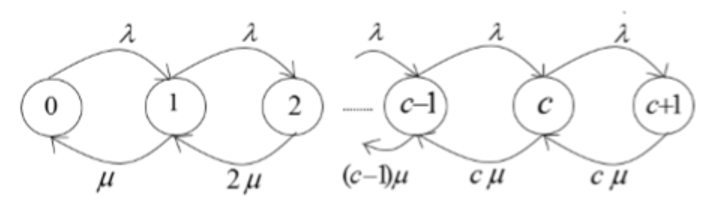
\includegraphics[scale=1]{img/MMCK.PNG}
    \end{center}
    \caption{Mô hình hệ thống xếp hàng M/M/C/K.}
    \end{figure}
\end{center}
Ta thiết lập được ma trận sinh sau:
\begin{align*} G=
    \begin{bmatrix}
        -\lambda_0 & \lambda_0 \\
        \mu_1 & -(\mu_1 + \lambda_1) & \lambda_1\\
        &\mu_2 & -(\mu_2 + \lambda_2) & \lambda_2\\
        & & {\boldsymbol{\ddots}} & {\boldsymbol{\ddots}} &{\boldsymbol{\ddots}}\\
        & & & & & \lambda_n\\
        & & & &  \mu_n & -\mu_n
    \end{bmatrix}
\end{align*}
\par Phân phối dừng của lượng người trong hệ thống bán vé là vectơ $\pi$ là nghiệm của hệ
\begin{align*}
    \begin{cases}
    \pi G = 0 \\
    \displaystyle\sum_{i=0}^{k+1} = 1
    \end{cases}
\end{align*}
Từ đó ta suy ra được phân phối dừng của hệ thống
\subsection{Các đại lượng của mô hình M/M/1/K}
\begin{enumerate}
    \item Số lượng khách hàng trung bình trong hệ thống $L$:
    \begin{align*}L=
        \begin{cases}
        \rho \frac{1+k.\rho^{k+1}-(k+1)\rho^k}{(1-\rho)(1-\rho^{k+1})}&,\qquad \rho \neq 1\\
        \frac{k}{2} &, \qquad\rho = 1
        \end{cases}
    \end{align*}
    \item Số lượng khách hàng trong xếp hàng $L_q$:
    \begin{align*}L_q=
        \begin{cases}
        L - \frac{\rho(1-\rho^k)}{1-\rho^{k+1}}&,\qquad \rho \neq 1\\
        \frac{k(k-1)}{2(k+1)} &,\qquad \rho = 1
        \end{cases}
    \end{align*}
    \item Thời gian trung bình của một khách hàng phải mất trong hệ thống $W_s$:
    \[W_s = \frac{L}{\lambda(1-p_k)}\]
    \item Thời gian trung bình của một khách hàng phải mất để xếp hàng $W_q$:
    \[W_q = W_s - \frac{1}{\mu}\]
    \item Tỷ lệ hoạt động có ích của hệ thống $\rho$: $\rho = \frac{\textit{dòng vào}}{\textit{dòng ra}}$
    \[\rho = \frac{\lambda}{\mu}\]
    \item Tỷ lệ thời gian nhàn rỗi của hệ thống $p_0$:
    \begin{align*}p_0=
        \begin{cases}
        \frac{1-\rho}{1-\rho^{k+1}}&,\qquad \rho \neq 1\\
        \frac{1}{k+1} &,\qquad \rho = 1
        \end{cases}
    \end{align*}
    \item Xác suất khi hệ thống phục vụ hết khách hàng $p_n$:
    \[p_n = p_0 . \rho^n\]
\end{enumerate}
\subsection{Các đại lượng của mô hình M/M/C/K}
\begin{enumerate}
    \item Số lượng khách hàng trung bình trong hệ thống $L$:
    \[L=L_q + c - p_0 \displaystyle\sum_{n=0}^{c-1} \frac{(c-n)(\rho c)^n}{n!}\]
    \item Số lượng khách hàng trung bình trong xếp hàng $L_q$:
    \[L_q = \frac{p_0 r^c \rho}{c!(1-\rho)^2}[1-\rho^{K-c+1} - (1-\rho)(K-c+1)\rho^{K-c}],\]
    trong đó $\rho = \frac{\lambda}{c\mu} \neq 1.$
    \item Thời gian trung bình của một khách hàng phải mất trong hệ thống $W_s$:
    \[W_s = \frac{L}{\lambda(1-p_k)}\]
    \item Thời gian trung bình của một khách hàng phải mất để xếp hàng $W_q$:
    \[W_q = \frac{L_q}{\lambda(1-p_k)}\]
    \item Cường độ dòng đến (dòng vào) $\lambda$: 
    \begin{align*} \lambda_n = 
        \begin{cases}
        \lambda \;\;&,\quad 0 \le n < k \\
        0 &,\quad n \ge k
        \end{cases}
    \end{align*}
    \item Cường độ dòng phục vụ (dòng ra) $\mu$: 
    \begin{align*} \mu_n = 
        \begin{cases}
        n\mu \;\;&,\quad 0 \le n < c \\
        c\mu &,\quad c \le n \le k
        \end{cases}
    \end{align*}
    \item Tỷ lệ thời gian nhàn rỗi của hệ thống $p_0$:
    \begin{align*}p_0 =
        \begin{cases}
        \Bigg[\displaystyle\sum_{n=0}^{c-1}\bigg(\frac{1}{n!}r^n \bigg) + \bigg(\frac{r^c}{c!}\bigg)\Bigg(\frac{1-\rho^{K-c+1}}{1-\rho}\Bigg)\Bigg]^{-1} &,\;\;\rho \neq 1 \\
        \bigg[\displaystyle\sum_{n=0}^{c-1}\bigg(\frac{1}{n!}r^n \bigg) + \bigg(\frac{r^c}{c!}\bigg)(K-c+1)\bigg]^{-1} &,\;\;\rho = 1
        \end{cases}
    \end{align*}
    \item Xác suất khi hệ thống phục vụ hết khách hàng $p_n$:
    \begin{align*}p_n =
        \begin{cases}
        \frac{1}{n!}(\frac{\lambda}{\mu})^n p_0  &,\qquad 0 \le n < c \\
        \frac{1}{c^{k-c}c!}(\frac{\lambda}{\mu})^n p_0 &,\qquad c \le n \le k
        \end{cases}
    \end{align*}
\end{enumerate}

\chapter{Chương trình }
Xây dựng chương trình trên nền tảng C#.NET giúp người dùng chỉ cần nhập những thông số input cơ bản của hệ thống sẽ đưa ra kết quả là Phân phối dừng và lợi nhuận thu được từ đó có thể đánh giá, cân nhắc đưa ra lựa chọn thay đổi hệ thống sao cho hợp lý.
\section{Một số mã nguồn chính}
    \subsection{Khởi tạo}
    \begin{my-itemize}
        \item mohinh.a - Dòng vào a (giá trị $\lambda$)
        \item mohinh.b - Dòng ra  b (giá trị $\mu$)
        \item mohinh.c - Số kênh c (giá trị $c$)
        \item mohinh.d - Số khách tối đa d (giá trị $k$)
        \item ln - Lợi nhuận
        \item L - Số khách trung bình toàn bộ hệ thống
    \end{my-itemize}
    
        \begin{flushleft}
     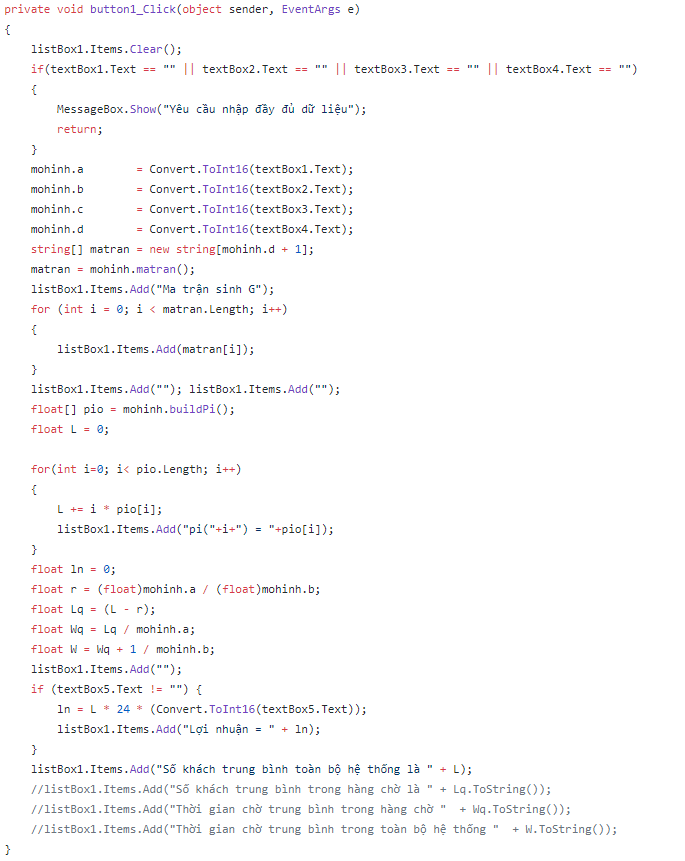
\includegraphics[scale]{img/khoitao.PNG}
\end{flushleft}
\subsection{Thiết lập ma trận sinh G}
Bài toán có $k+1$ trạng thái\[\lambda_i = \lambda, \forall i = 1,2,...,n\]
\begin{align*}
    \mu_n = \begin{cases}
    n\mu, \qquad n=1,2,...,c-1\\
    c\mu, \qquad n=c,c+1,...
    \end{cases}
\end{align*}
Ta thiết lập được ma trận sinh sau:
\begin{align*} G=
    \begin{bmatrix}
        -\lambda_0 & \lambda_0 \\
        \mu_1 & -(\mu_1 + \lambda_1) & \lambda_1\\
        &\mu_2 & -(\mu_2 + \lambda_2) & \lambda_2\\
        & & {\boldsymbol{\ddots}} & {\boldsymbol{\ddots}} &{\boldsymbol{\ddots}}\\
        & & & & & \lambda_n\\
        & & & &  \mu_n & -\mu_n
    \end{bmatrix}
\end{align*}
\begin{flushleft}
     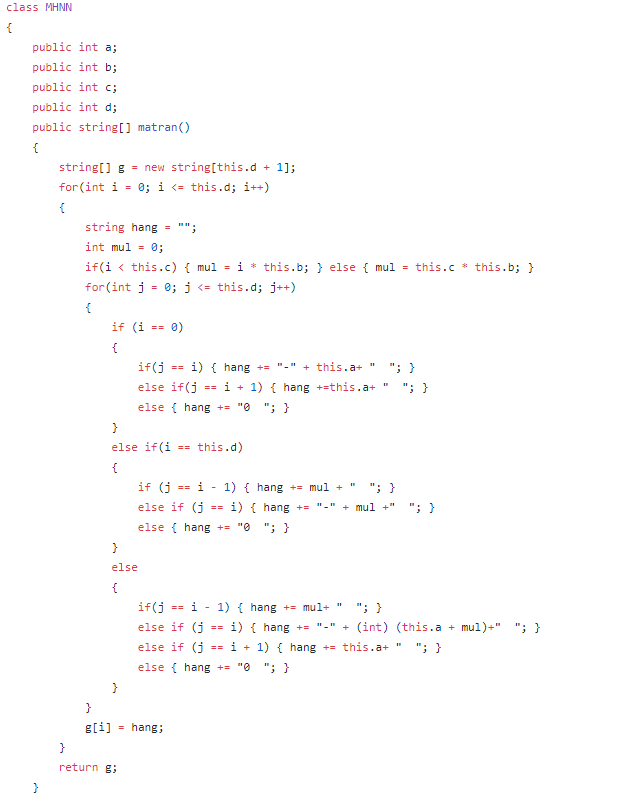
\includegraphics[scale]{img/mtsinhG.PNG}
\end{flushleft}
\subsection{Tìm phân phối dừng $\pi_i$}
Phân phối dừng là nghiệm của hệ:
\begin{align*}
    \begin{cases}
    \pi.G &= 0\\
    \pi_0 \lambda_0 &=\pi_1 \mu_1\\
    \pi_1 \lambda_1 &=\pi_2 \mu_2\\
    ...\\
    \pi_{k-1} \lambda_{k-1} &=\pi_k \mu_k\\
    \end{cases}
\end{align*}
trong đó $\lambda_i = \lambda, \forall i$. Ta tính các $\pi_i, \forall i > 0$ theo $\pi_0$.\\
Tiếp đến ta thay $\pi_i$ theo $\pi_0$ vào biểu thức điều kiện:$\displaystyle\sum_{i=0}^{k}\pi_i = 1$\\
Ta thu được $\pi_0 = \frac{1}{1 + tong}$
với giá trị: \[tong = \frac{\lambda}{\mu_1}+\frac{\lambda.\lambda}{\mu_1.\mu_2}+...+\frac{\lambda^k}{\mu_1.\mu_2...\mu_k}\]
Cuối cùng ta tính các đại lượng bởi công thức:
\[\pi_n =\frac{\lambda}{\mu_n}\pi_{n-1}, \qquad \text{với} n = 1,2,...,k\]
$\Longrightarrow \pi_1 = \frac{\lambda}{\mu_1}\pi_0;\;\;\; \pi_2 = \frac{\lambda}{\mu_2}\pi_1;\;\;....\;\;;\;\;\;\pi_k =\frac{\lambda}{\mu_k}\pi_{k-1}$
\begin{flushleft}
     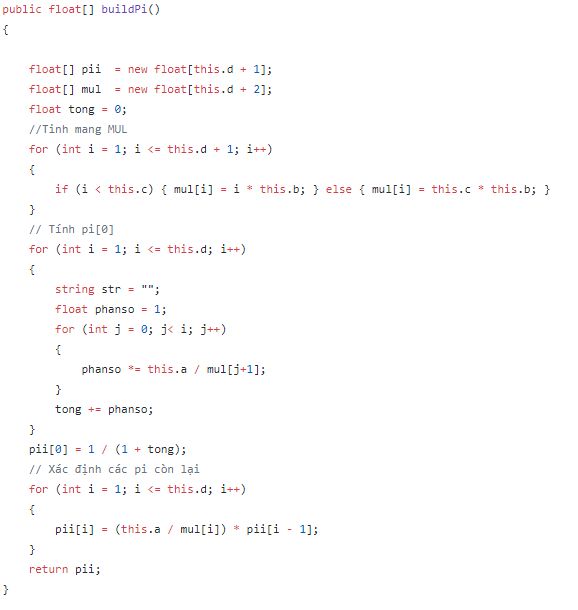
\includegraphics[scale]{img/ppdung.PNG}
\end{flushleft}
\end{enumerate}
\subsection{Tính số khách trung bình toàn bộ hệ thống}
Công thức áp dụng:
\[L = \displaystyle\sum_{i=0}^{k} i.\pi_i\]
\begin{flushleft}
     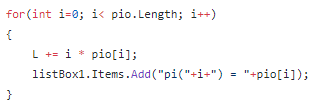
\includegraphics[scale]{img/TinhL.PNG}
\end{flushleft}
\subsection{Lợi nhuận}
Công thức áp dụng: Tính lợi nhuận sau 24 giờ khi có lợi nhuận đầu vào
\[\textit{Lợi nhuận}= \textit{Lợi nhuận}_{input} * 24 * L\]
\begin{flushleft}
     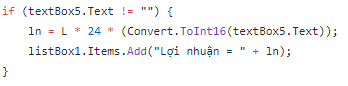
\includegraphics[]{img/TinhLoiNhuan.PNG}
\end{flushleft}
\newpage
\section{Chạy chương trình}
\begin{center}
    \begin{figure}[htp]
    \begin{center}
     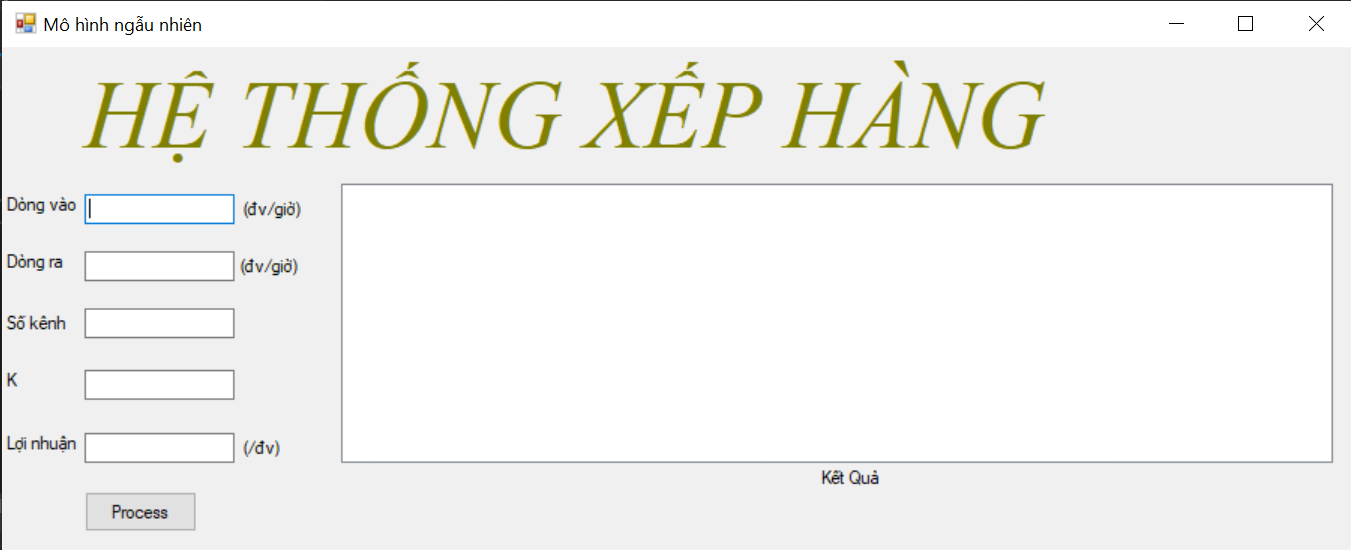
\includegraphics[scale=.7]{img/giaodien1.PNG}
    \end{center}
    \caption{Giao diện khi chưa input}
    \end{figure}
    \begin{figure}[htp]
    \begin{center}
     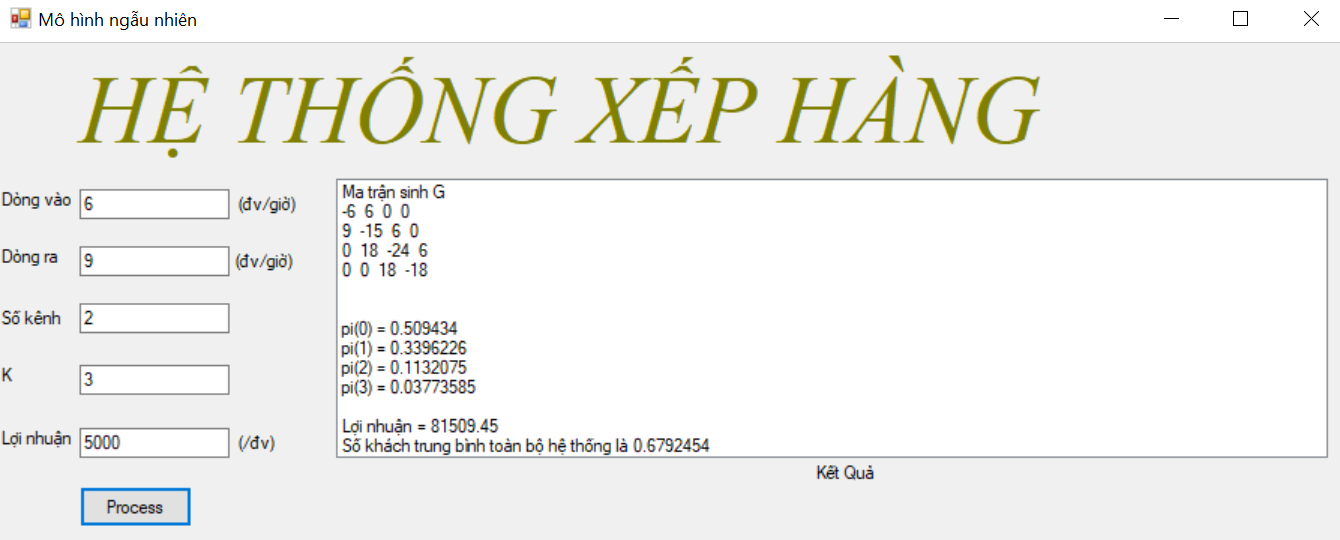
\includegraphics[scale=.7]{img/giaodien2.PNG}
    \end{center}
    \caption{Giao diện khi đã input}
    \end{figure}
\end{center}

\\
\\
Mã nguồn đầy đủ:\par
\url{https://github.com/NguyenThienDong/MHNN}
\chapter*{Kết luận}
Việc xây dựng mô hình mô phỏng trong thực tế là rất khó khăn và phức tạp. Lý thuyết xếp hàng có nhiều ứng dụng quan trọng trong việc phân tích và giải quyết một số bài toán thực tế. Trong tiểu luận này nhóm em đã cố gắng áp dụng quá trình sinh-tử của lý thuyết hàng chờ để giải quyết một vấn đề nhỏ trong bài toán bán vé tàu. Tuy nhiên, vì thời gian có hạn, sự am hiểu về môn học còn hạn chế nên nội dung còn nhiều thiếu sót.  Nguyện vọng tiếp theo của bản thân là cố gắng tìm hiểu sâu hơn về Lý thuyết xếp hàng cùng với các ứng dụng thực tế và đa dạng hơn. Một lần nữa chúng em xin chân thành cảm ơn cô giáo TS. Nguyễn Thị Ngọc Anh đã giúp chúng em trong quá trình tiếp cận môn học và thực hiện tiểu luận này.
\addcontentsline{toc}{chapter}{{\bf Kết luận}\rm}

\begin{thebibliography}{}
\bibitem{}Ngô Hoàng Long, \textit{Mô hình ngẫu nhiên và ứng dụng., }, 2018.
\bibitem{} Trần Lộc Hùng, \textit{Bài giảng Mô phỏng ngẫu nhiên (Cao học CNTT)}, Huế, 2007.
\bibitem{} Trần Lộc Hùng, \textit{Bài giảng Mô phỏng ngẫu nhiên (Cao học CNTT)}, Huế, 2007.
\bibitem{} Đặng Hùng Thắng, \textit{Quá trình ngẫu nhiên và tính toán ngẫu nhiên}, Nhà
xuất bản Đại học quốc gia Hà Nội, 2007.
\end{thebibliography}
\addcontentsline{toc}{chapter}{{\bf Tài liệu tham khảo}\rm}
\end{document}
